% Social Media Analytics 2022/23

%%%%%%%%%%%%%%%%%%%%%%%%%%%%%%%%%%%%%%%%%%%%%%%%%%%%%%

% OPTIONAL PACKAGES
\documentclass[12pt,journal,compsoc]{IEEEtran}
\usepackage{amsfonts}
\usepackage{caption}
\usepackage{multirow}
\usepackage[table,xcdraw]{xcolor}
\usepackage{booktabs}
\usepackage{tabularx}
\usepackage[hyphens]{url}
\usepackage{biblatex}
\usepackage{blindtext,graphicx}
\usepackage[absolute]{textpos}
\usepackage[italian]{babel}
\usepackage{float}
\usepackage{hyperref}
\addbibresource{ref.bib} %Import the bibliography file

%%%%%%%%%%%%%%%%%%%%%%%%%%%%%%%%%%%%%%%%%%%%%%%%%%%%%%

\begin{document}

\begin{textblock}{5}(1,0.5)
\noindent\small Social Media Analytics - UniMib 2022/23
\end{textblock}

\title{Smart Working\\
\vspace{2mm}\large{Social Network and Content Analysis}}
\author{Agazzi Ruben 844736\\Cominetti Fabrizio 882737}

\IEEEtitleabstractindextext{%
\begin{abstract}
In recent years, the topic related to \textit{smart working} has taken a prominent place in work-related discussions. From the need during the pandemic period to the demands of workers who, once the post-pandemic health situation was reestablished, did not want to give up this option, which was considered an advantage in their work-life balance. But the topic is also discussed because of the benefits to companies, especially in terms of saving on facilities and energy, or again because of traffic and pollution issues. In short, smart working can no longer be considered a second-rate issue. For this reason, we wanted to analyze user sentiment and communities with regard to the topic, especially after the latest interventions at the government level that have partially reduced the possibility of taking advantage of smart working.
\end{abstract}}

\maketitle
\IEEEpeerreviewmaketitle
\IEEEdisplaynontitleabstractindextext

\tableofcontents

%%%%%%%%%%%%%%%%%%%%%%%%%%%%%%%%%%%%%%%%%%%%%%%%%%%%%%

\section{Introduction}
\IEEEPARstart{S}{mart} Working, also known as agile working, means \textit{a mode of execution of the employment relationship characterized by the absence of hourly or spatial constraints and an organization by phases, cycles and objectives, established by agreement between employee and employer; a mode that helps the employee to reconcile work and life times and, at the same time, encourage the growth of his or her productivity} \cite{Gazzetta} \cite{MIUR}.
Smart working is an organizational model that can bring significant benefits to organizations that adopt it: in terms of productivity, goal achievement, but also in terms of worker welfare and quality of life.\\
As early as 2015, the British Standards Institution stated that: \textit{"The principles of smart working recognize that technology and flexible working models are changing the way we work for the better} \cite{BSI}.\\
Looking at the other side of the coin, research such as that conducted by NordVPN in 2020 has uncovered some risks for workers, including an unintended increase in working hours, isolation of the individual and the individual's difficulty in separating social life and work activity, as well as dangers related to privacy and security issues \cite{Forbes}.\\
Between the end of 2021 and the beginning of 2022, there were an estimated 2.9 million so-called "smart workers" in Italy, up from 1.15 million at the end of 2019 but down nowadays and out of an estimated total of 8 million potential users. The same research also shows that Italy is at the bottom of the list in the adoption of smart working in Europe and has a far lower average than the EU average considering number of individuals and total days per week of agile work \cite{Rai}.\\
Starting in February 2020, following the spread of the Covid-19 outbreak of the Coronavirus epidemic, a series of measures were issued by the government to simplify access to Smart Working and spread its use as much as possible. Indeed, the pandemic has forced many workers to cope with the health emergency through smart working.\\
The numbers enunciated above suggest that once the toughest phase of the emergency was over - with measures including lockdown - most companies and workers chose to return to traditional ways of working.\\
Public opinion is divided between those who preferred to continue using an agile work mode afterwards, pointing out its many benefits, and those with an opposing view who support the importance of face-to-face communication and consider daily human interaction irreplaceable, or would still like to give way to new tools and technologies.\\
In addition to all this, it should also be pointed out that only certain types of workers can continuously carry out an agile work mode, mainly office workers, while others thus have a marginal interest in the topic.\\
In addition to the aforementioned pandemic, the attached directives for workers and the various extensions to the state of emergency and smart working under a simplified regime have once again brought the phenomenon to the forefront.\\
Indeed, the government extended in the last days of 2022 the right to smart working with a dedicated amendment in the Maneuver only for workers considered "fragile" in the public and private sectors. So, saying goodbye to work-from-home days for parents of children under 14, until before this amendment included in the measure passed by the previous Executive, and who from January 1 had to go back to individually bargaining remote work days with their company.\\
The government's decision to exclude parents of children under 14 from the measure is explained by the demise of the anti-Covid measures adopted during the pandemic, on which the need for remote work for millions of workers was based.\\
Our analysis therefore wants to focus on this final period, between the end of 2022 and the beginning of 2023, to investigate the reactions, sentiment, and emotions poured onto the network - Twitter in our case - following the announcement of these decisions.\\
In conclusion, the project aims to answer questions such as \textit{How is the Italian landscape represented around the issue on Twitter? Who are the most influential users within it? What was the general sentiment during the period under consideration? What were the emotions and different reactions in the days around the government's announcement on the further reduction of Smart Working}?

\section{Data Collection}
To build the dataset, which is needed to answer the project questions, we downloaded a total of 2667 tweets from the social network Twitter, through the use of the API provided by the social.\\
The data were downloaded using a jupyter notebook and the Tweepy library, which allows downloading tweets corresponding to one or more hashtags or keywords. In our case, we chose to use the following keywords: \textit{"smartworking" OR "remotework" OR "lavoroagile" OR "smart working" OR "remote work" OR "lavoro agile"}.\\
Since the topic is debated and particularly concerns Italy, we chose to conduct the study on Italian-language tweets, thus downloading only tweets in the selected language.\\
The API allows downloading tweets with some limitations related to the number of days and consecutive download requests. The period of interest is from December 26, 2022 to January 5, 2023. Thus, the period also considers initial days when some rumors about it were beginning to emerge and a later period after the official announcement. As we can observe from the following distribution, the day with the highest number of tweets posted is December 30, 2022, the penultimate day of agile work granted also to parents of U14 children and the day when the - obligatory - option to return to the office was getting closer and closer for many Italians. But not only that, because on the same day a circular by 'Ministero della Salute' announced the return to smart working only in case of worsening health situation.

\begin{figure}[H]
  \begin{center}
  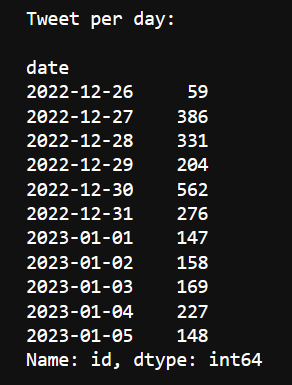
\includegraphics[scale=1]{./images/tweetxday.png}
  \end{center}
  \caption{Number of Tweets per Day}
\end{figure}

The initial dataset, exported and saved in csv, thus consists of a total of 10 variables: \{date, id, text, like, n\_rt, author, location, retweeted, user\_mentions, hastags\}.

\begin{itemize}
	\item \textit{date}: date and time the tweet was published
	\item \textit{id}: unique identifier of the tweet
	\item \textit{text}: text contained in the tweet, extracted via the extended option
	\item \textit{like}: number of likes
	\item \textit{n\_rt}: number of retweets
	\item \textit{author}: username of the author of the tweet
	\item \textit{location}: location of tweet posting, not always available
	\item \textit{retweeted}: Boolean value, 'true' if it is a retweet, 'false' otherwise
	\item \textit{user\_mentions}: mentions of other users contained in the tweet
	\item \textit{hastags}: hashtags used in the tweet
\end{itemize}

\subsection{Data Pre-Processing}
The first operation performed was to check for duplicates, and subsequent removal of duplicates. No duplicate tweets are present, so the total number of tweets remains at 2667 items.\\
The format of the variable 'date' was processed and the variables 'day', 'month', and 'year' were extracted to display the number of tweets made per day, as seen in the image above.\\
After that, we created a dataframe within which a count of number of tweets made by the same author was performed. The result can be seen in the image and the table below:

\begin{figure}[H]
  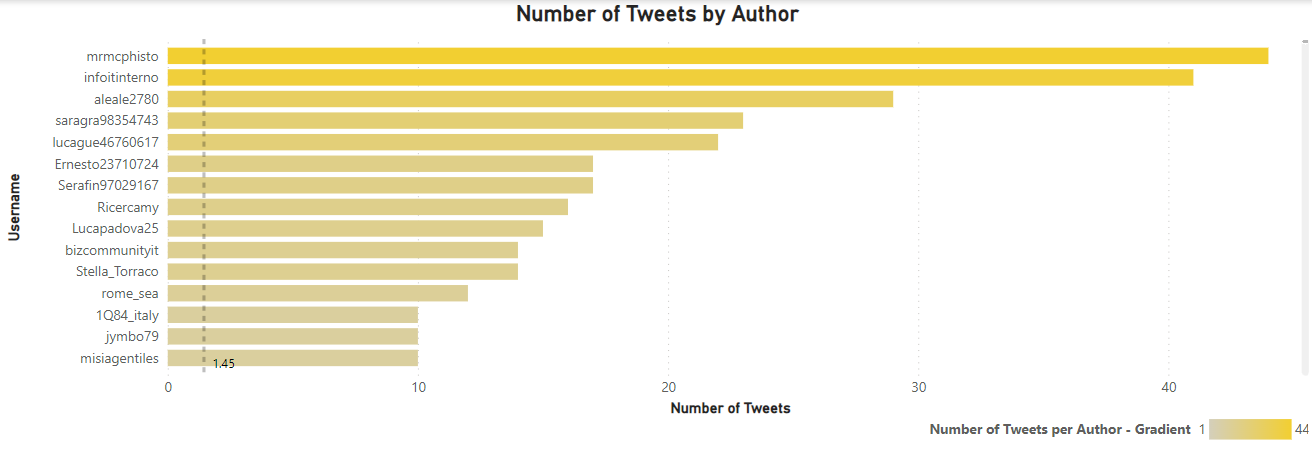
\includegraphics[scale=0.4]{./images/tweetsxauthor.png}
  \caption{Number of Tweets by Author}
\end{figure}

\begin{table}[ht]
\centering
\begin{tabular}{c c }
	Username & Num of Tweets  \\
	\hline
	mrmcphisto & 44  \\
	infoitinterno & 41  \\
	aleale2780 & 29  \\
	saragra98354743 & 23  \\
	lucague46760617 & 22  \\
\end{tabular}
\caption{First five authors ordered by number of Tweets}
\end{table}

From each tweet, we then extracted the list of hashtags and mentions contained, placed in two columns of the main dataframe, respectively: \{hashtags\_list, mentions\}.\\
For each document in the corpus, the pre-processing operations necessary to analyze the text were performed. Specifically:

\begin{itemize}
	\item \textit{Remove Numbers} : removal of numbers within the text
	\item \textit{Lower Text} : text converted to lowercase
	\item \textit{Lemmatization} : grouped together the various forms of a word so they can be analysed as a single item, identified by the word's lemma
	\item \textit{Remove Punctuation} : removal of punctuation elements
	\item \textit{StopWords Deletion} : removal of Italian stopwords
	\item \textit{Tokenization} : each text has been tokenized
\end{itemize}

\section{Analysis}

\subsection{Social Network Analysis}
For the social network analysis we took the dataset of tweets we obtained from the twitter web api, and we kept only the columns relative to the tweet's author username and the list of users mentioned in the tweet.
 
\subsubsection{Graph building}
We built our graph using the python library "NetworkX\cite{NetworkX}". Specifically we took every tweet in our dataset and for every tweet we took the tweet's author and users mentioned in the tweet, which becomes nodes of the graph, and then we make an edge between them. After this step we created inside our graph a total of 1820 nodes and 2568 edges between nodes.

\subsubsection{Nodes degree}
After building the graph we calculated the degree of every node inside the graph. The degree of a node of a graph is the number of edges that are incident to the node. After calculating the degree for every node we found out that the maximum degree found inside the graph is equal to 210 and the minimum degree found is equal to 1. 
\begin{table}[ht]
\centering
\begin{tabular}{c c }
	Node name & Degree  \\
	\hline
	BonomiAllegra & 210  \\
	mrmcphisto & 145  \\
	GiorgiaMeloni & 141  \\
	AlbertoBagnai & 118  \\
	ClaudioDurigon & 82  \\
\end{tabular}
\caption{First five nodes ordered by degree}
\end{table}
We also decided to calculate the average degree of the graph, which is equal to 2.82. Because the average degree is greater than 1 we already assumed that there will be a giant component inside the graph. A giant component in graph theory is a connected component of a graph that contains a finite fraction of the entire graph's vertices.

\subsubsection{Assortativity}
Assortativity is a measure of how nodes inside a network connect to each other. If an interaction network is assortative nodes of comparable degree tent to link each other: bigger nodes(hubs) will tend to connect to hubs and smaller nodes will tend to connect to each other. If an interaction network is disassortative hubs wille tend to connect to small degree nodes, and small degree nodes will tend to connect to hubs. If the interaction network is neutral nodes will link to each other randomly.\\
We can calculate an assortativity coefficient of a graph; if this coefficient is greater than 0 the network is assortative, if is equal to 0 is neutral and if is less than 0 it is disassortative.
In out case the assortativity coefficient is equal to -0.244, which makes our network disassortative.

\subsubsection{Community detection}
Communities are parts of the graph that are more densly connected, meaning they interact a lot with each other. In this case we used the python library "NetworkX\cite{NetworkX}" to find the community with modularity maximization. Local modularity is based on the hypothesis that random network does not have comunities. Local modularity\cite{Modularity} compares the number of links between the real network and the one expected on a random network. We can calculate the local modularity in the following way:
\[M_c = \frac{1}{2L}\sum_{i \in C, j\in C }(A_{ij} - \frac{d_id_j}{2E})\] 
Where:
\begin{itemize}[]
    \item $A_{ij}$: Is the actual number of edges between nodes i and j.
    \item $\frac{d_id_j}{2E}$: is the expected number of edges in a random network for nodes i and j.
\end{itemize}
If the modularity is less than zero the network is randomly connected, and if the modularity for a community of nodes is less than zero then it is not considerable as a community.
After running the modularity maximization algorithm we found 197 different communities, and the biggest community is formed by 234 nodes.
\begin{table}[ht]
	\centering
	\begin{tabular}{c c }
		Community number & Number of nodes  \\
		\hline
		Community 0& 234  \\
		Community 1& 210  \\
		Community 2& 179  \\
		Community 3& 139  \\
		Community 4& 87  \\
	\end{tabular}
	\caption{First 5 communities by node count}
	\end{table}
	
\subsubsection{Visualizations}
\begin{figure}[H]
	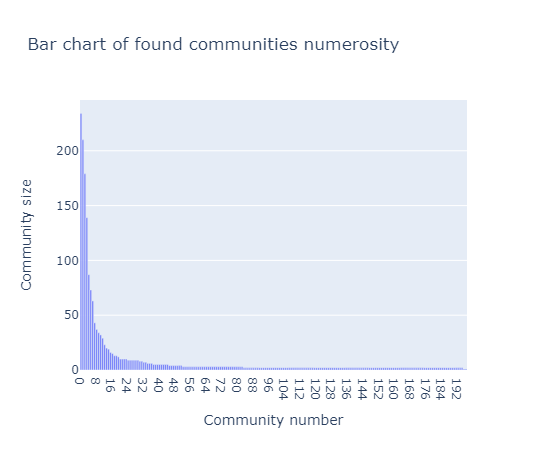
\includegraphics[scale=.5]{./images/newplot.png}
	\caption{Bar chart of the communities numerosity.}
\end{figure}

\begin{figure}[H]
	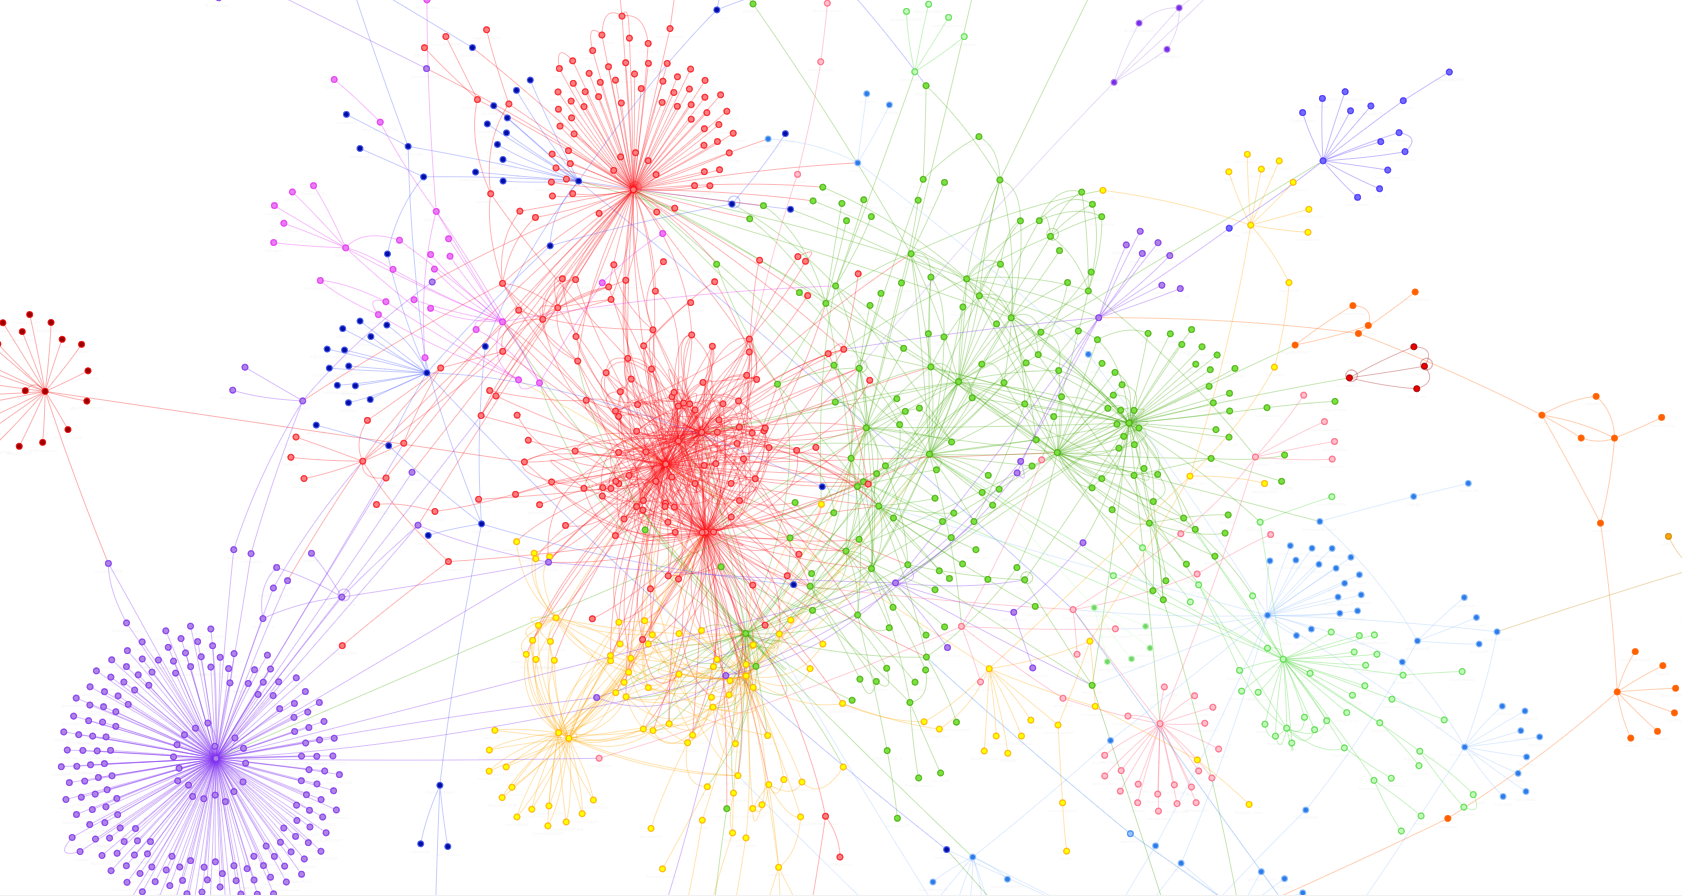
\includegraphics[scale=.20]{./images/graph_visualization.png}
	\caption{Visualization of part of the graph with different colors representing different communitites.}
\end{figure}

\subsection{Social Content Analysis}
As for the \textit{Social Content Analysis}, FEEL-IT, a dataset and package was used to carry out \textit{Sentiment Analysis} and \textit{Emotion Recognition} in the Italian language.\\
BERT is one of the most popular neural architectures in Natural Language Processing, and FEEL-IT \cite{FEEL-IT}, available in Python, takes advantage of the model (Um)BERT(o), a very efficient Italian BERT model, optimized and fine-tuned.

\subsubsection{Sentiment Analysis}
Regarding \textit{Sentiment Analysis}, the package divides the tweets into 'positive' and 'negative,' values that were assigned to a new column, called 'sentiment\_BERT.' In addition, depending on the value assigned by the model, three other variables were created, 'positive', 'negative', with value 1 in case of value matching sentiment (thus 1 to the 'positive' column in case of identified positive sentiment) and 0 otherwise, and 'ratio', with value 1 in case of positive sentiment and -1 in case of negative sentiment. The dataset thus composed was saved in a csv file for further analysis.\\
The image below reveals the division of tweets between positive and negative sentiment. As we can see, the negative sentiment clearly outweighs the total percentage, coming in at over 85\%. The result could have been considered expected, but the percentage is certainly high.

\begin{figure}[H]
\begin{center}
  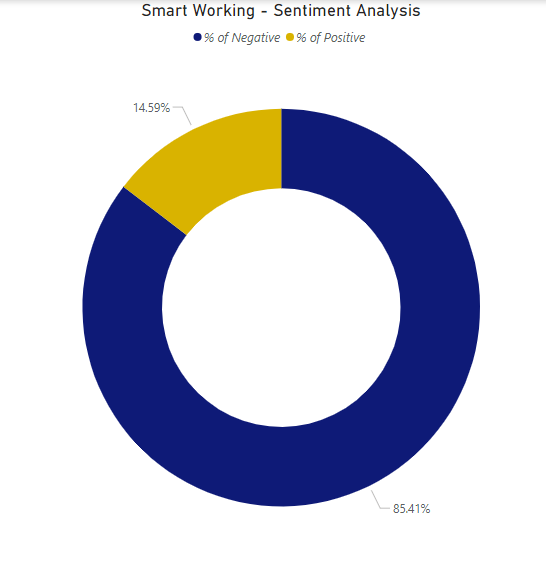
\includegraphics[scale=0.7]{./images/pie-sentiment.png}
\end{center}  
  \caption{Sentiment - Positive and Negative percentage}
\end{figure}

Considering the sentiment on the various days, it can be seen that it is highly negative on some dates. In particular on 30/12, the day on which a Ministry of Health circular enunciated the plan to encourage smart working only in the event of a worsening health situation. News that, as we can observe, did not leave the workers involved satisfied.

\begin{figure}[H]
  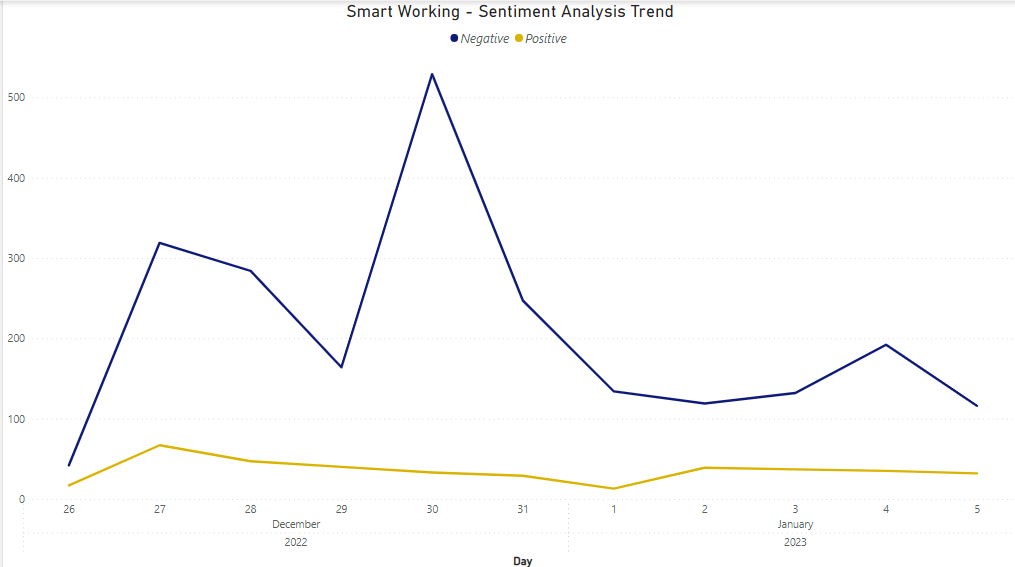
\includegraphics[scale=0.5]{./images/trend-sentiment.png}
  \caption{Sentiment - Daily Trend}
\end{figure}
\subsubsection{Emotion Recognition}
Recognizing emotions in text is fundamental to get a better sense of how people are talking about something. People can talk about a new event, but positive/negative labels might not be enough. There is a big difference between being angered by something and scared by something. This difference is why it is vital to consider sentiment and emotion in text.\\
The model of \textit{Emotion Recognition} is able to identify four emotions: 'joy', 'fear', 'anger', 'sadness'. The procedure carried out is the same for sentiment analysis, and thus four variables were created, one for each emotion, with value 1 in case of tweets corresponding to the same emotion, 0 otherwise. Again, the dataset was exported to a csv file for further analysis.

\begin{figure}[H]
  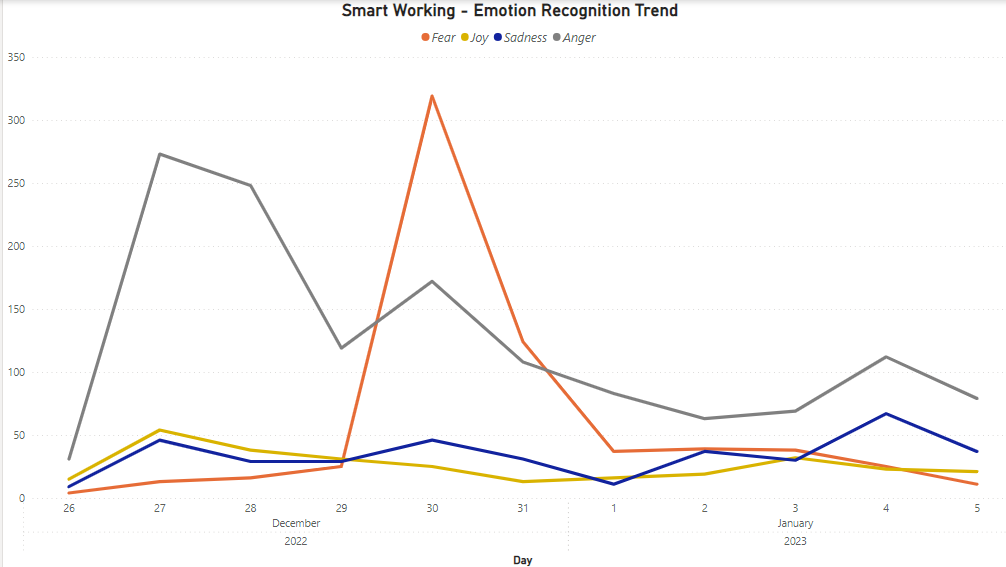
\includegraphics[scale=0.5]{./images/trend-emotion.png}
  \caption{Emotion - Daily Trend}
\end{figure}

As we can observe from the historical series above, the emotion 'fear' has a peak on the day of 30/12. The emotion 'anger' is definitely the most prevalent over the historical series, while 'joy' and 'sadness' are almost constant.

\section{Summary}
The project carried out allowed us to investigate the research questions we had set, both regarding the network analysis part and the content analysis part.\\
We undurstood that even with a relatively small number of nodes (1820) with the right topic is very easy to form communities inside a social network.\\
We also understood from the sentiment analysis that the 'anger' emotion is the most prevalent regarding this subject.
Future developments of the project could consider a wider range of days, or use (design) a sentiment classification model that considers a neutral value of some texts. We could also consider analyzing different community detection algorithms in order to see how differently they identify the various communities.

%%%%%%%%%%%%%%%%%%%%%%%%%%%%%%%%%%%%%%%%%%%%%%%%%%%%%%%%%%%%%%%%%

\nocite{*}
\printbibliography

\end{document}